\cotefile{23}
\scanpage{2}
EGA $\overline{\underline{\mathrm{IV}}}$, Calcul diff. (compléments)
% archive sheet number: 1

\scanpage{3}
\unsure{Discriminant|Discriminants} etc
% archive sheet number: 2

\scanpage{4}
$E$ faisceau loc. libre de rang $r+1$ sur $S$

$P=\mathrm{P}(E)$ fibré projectif associé, on a une suite exacte canonique
\[
0\longrightarrow\Omega^1_{P/S}\longrightarrow g^*(\underline E)(-1)\longrightarrow\underline O_P\longrightarrow0
\]
[qui donne un isom can
\[
\Omega^r_{P/S}\xrightarrow{\sim}g^*\bigl(\bigwedge_{\underline O_S}^{r+1}E\bigr)(-r-1)\tag*{(1)}
\]
\hfill$]$

Si \unsure{donc} $X$ est un sous-préschéma de $P$ \unsure{simple|lisse} sur $S$, de dim relative \inserted{$n=$}$r-p$
associé au faisceau \deleted{loc. libre}\inserted{d'idéaux} $J$, on a la suite exacte
\[
0\longrightarrow J/J^2\longrightarrow\Omega^1_{P/S}\otimes\underline O_X\longrightarrow\Omega^1_{X/S}\longrightarrow0
\]
d'où l'isomorphisme
\[
\Omega^r_{P/S}\otimes\underline O_X\xleftarrow{\sim}\Omega^{\deleted{\unsure{r-p}}\unsure{n}}_{X/S}\otimes\bigwedge^p_{\underline O_X}(J/J^2)\tag*{(2)}
\]
d'où en composant (1) et (2), désignant par $f:X\to S$
le morphisme structural
\[
\deleted{\Omega^r}f^*\bigl(\bigwedge_{\underline O_S}^{r+1}\underline E\bigr)(-r-1)\xleftarrow{\sim}\Omega^{\deleted{\unsure{r-p}}\unsure{n}}_{X/S}\otimes\bigwedge^p_{\underline O_X}(J/J^2)
\]

Supposons que $X$ soit une intersection complète, définie
par un sous-module \inserted{gradué $M$ \deleted{\unsure{de|\(\subset\)}}} loc. facteur direct de $\mathrm{Symm.}^{*}(\underline E)$,
\deleted{\unsure{qui soit de rang}} loc. libre de rang $p$ [il n'est \deleted{de fait}
déterminé que modulo le carré $\underline I^2$ de l'idéal qu'il
définit ; mais sa structure est connue]. On a
un hom, si $I_a$ est la composante de degré $a$ de $I$
\[
g^*(I_d)(-d)\longrightarrow J
\]
d'où des hom \uline{surjectif}
\[
\coprod g^*(M_d)(-d)\longrightarrow J
\]
induisant un \uline{isom}
\[
\coprod f^*(M_d)(-d)\xrightarrow{\sim}J/J^2\simeq\mathrm{Conormal}_{P/X}
\]
% archive sheet number: 3

\scanpage{5}
Par suite, on a
\[
\bigwedge_{\underline O_X}^p J/J^2\simeq f^*\bigl(\bigotimes_i\bigwedge^{\alpha_i} M_{d_i}\bigr)(-\sum\alpha_i d_i)
\]
ou $M_{d_i}$ sont les composantes \unsure{non|des} nulles de $M$, supposées
de degré $\alpha_i$. D'où un isom
\[
\Omega^n_{X/S}\otimes f^*\bigl(\bigotimes_i\bigwedge^{\alpha_i}M_{d_i}\bigr)(-\sum\alpha_i d_i)
\xrightarrow{\sim}f^*\bigl(\bigwedge_{\unsure{\underline O_S|S}}^{r+1}\underline E\bigr)(-r-1)
\]
[\unsure{correspondant à|correspondant :|Correspondant :} un hom qui existe en tous cas dès
qu'on se donne des $M_{d_i}\longrightarrow\mathrm{Symm}^{d_i}(\underline E)$, les $M_{d_i}$ loc.
libres de rang $\alpha_i$, et $X$ défini par \deleted{les}\inserted{l'idéal engendré par les} images
des $M_{d_i}$, posant $p=\sum\alpha_i$, $n=r-p$], i.e. on a
\[
\Omega^n_{X/S}\xrightarrow{\sim}f^*\bigl((\bigwedge_S^{r+1}E)\otimes(\bigotimes_i\bigwedge^{\alpha_i}\check M_{d_i})\bigr)(\sum\alpha_i d_i-r-1)
\]

Dans le cas où
\[
\sum\alpha_i d_i=r+1
\]
on trouve donc
\[
\Omega^{\unsure{n}}_{X/S}\xrightarrow{\sim}f^*(\,-\,)
\]

Supposons p.ex. que $E$ soit le faisceau loc. libre de
rang $3$ associé à une courbe elliptique lisse
sur $S$, donc $r=2$, il n'y a qu'un seul $M_{d_i}$, $d_i=3$,
$\alpha_i=1$, on trouve
\[
\Omega^1_{X/S}\xrightarrow{\sim} f^*(\bigwedge^3 E\otimes\check M)
\]
Or $E$ a une filtration de facteurs $\underline O_S$, $\deleted{\unsure{g|L}}\mathcal L^{\otimes2}$, $\mathcal L^{\otimes3}$,
où $\mathcal L$ est un module inv tel que $f^*(\mathcal L)\simeq\unsure{\mathfrak g|\mathfrak T|\mathscr T|\mathcal T}_{X/S}$, donc
$\bigwedge^3 E\simeq\mathcal L^{\otimes5}$, et comme $\Omega^1_{X/S}\simeq f^*(\check{\mathcal L})$, on aura
$\check{\mathcal L}\xrightarrow{\sim}\mathcal L^{\otimes5}\otimes\check M$ d'où $M\xrightarrow{\sim}\mathcal L^{\otimes6}$.
% archive sheet number: 4

\scanpage{6}
\diagram{\(\begin{array}{ll}
 E & \mathrm{Symm}_k(E^{\deleted{\unsure{\vee}}})^\vee\\
 P^r & \Phi^k(P^r).
\end{array}\)}
\margin{$\underbrace{k-1\quad k-1\qquad k-1}_{r+1\ \text{fois}}$}

\[
\deleted{\unsure{g}}\delta_{r,k}\in\Phi^{(k-1)(r+1)}\bigl(\Phi^k(P^r)\bigr)
\]
\margin{$(k-1)(r+1)$}
(discriminant) défini au signe près

Section de $\underline O_{\Phi^k(P^r)}((k-1)(r+1))$

Considérons une section \inserted{$\varphi$} de $\Phi^k(P^r)$ sur $S$, elle
définit donc une \deleted{\unsure{hom|homom.} $\Phi^k(P^r)$ section du}
faisceau inversible $\check M$ sur $S$,
% slanted
\margin{quotient de $\mathrm{Symm}_k(E)^\vee$ \unsure{sol.|i.e.} dual \unsure{ou|du} sous faisceau \unsure{qu'on prend} $M$ de $\mathrm{Symm}_k(E)$}
image inverse
de $\underline O_{\Phi^k(P^r)}(1)$] et \deleted{si l'image la section
est inversible par la} \inserted{$\delta_{r,k}$ a comme}
image réciproque une section $\underset{\vee}{\delta}$ de
$\check M^{(k-1)(r+1)}$. Dire la section $\varphi$ ne rencontre
pas $\Phi^k(P^r)_{\delta_{r,k}}$, i.e. $P^r_\varphi$ est simple sur $S$,
sss $\delta$ est partout non nulle. Notons que
d'ailleurs, si $J=J_\varphi$ est l'idéal défini par $\varphi$
sur $P^r$, alors
\[
J\deleted{\unsure{_\varphi}}\simeq g^*(M^{\deleted{\unsure{\vee}}})(-k)
\]
\margin{\deleted{\unsure{identifier|identifions} \unsure{ci-contre} $M$ -- $\check M$}}
\[
\begin{aligned}
[\,\deleted{O(-k)\otimes g^*(E)\to}\quad &\underline O(-k)\otimes g^*(\mathrm{Symm}_k(E))\longrightarrow\underline O_{P^r}\\
\text{d'où}\quad &\underline O(-k)\otimes g^*(M)\longrightarrow\underline O_{P^r}\quad -\,)
\end{aligned}
\]
\margin{\unsure{pour le} choix d'un}
% archive sheet number: 5

\scanpage{7}
\mspage{3}
\[
\partial_\gamma\zeta_i^\beta(z,t)=\sum_{\mu=1}^n
\frac{\partial h_{ij}^\beta}{\partial\zeta_j^\mu}\cdot\partial_\gamma\zeta_j^\mu(z,t)\ .
\]

Comparing these equalities with (2) we infer immediately that
\[
\varphi_i^\beta(z,t)=\varphi_j^\beta(z,t),\qquad\text{for}\quad z\in U_i\cap U_j.
\]
Thus, letting
\[
\varphi(t)=(\varphi^1(t),\ldots,\varphi^\beta(t),\ldots,\varphi^n(t)),\quad
\varphi^\beta(t)=\varphi_j^\beta(z,t)\ ,
\]
we obtain a \uline{vector} $(0,1)$-\uline{form} $\varphi(t)$ on $V_0$ depending
differentiably on $t$. Since $\bar\partial\bar\partial\zeta_j^\beta(z,t)=0$, it follows from
(2) that
\[
\bar\partial\varphi^\beta(t)-\sum_{\gamma=1}^n\varphi^\gamma(t)\wedge\partial_\gamma\varphi^\beta(t)=0,\qquad
(\beta=1,2,\ldots,n),\tag*{(3)}
\]
where $\wedge$ denotes exterior multiplication of forms and
\[
\partial_\gamma\varphi^\beta(t)=\sum_\nu\partial_\gamma\varphi_{\bar\nu}^\beta(z,t)\,\mathrm d\bar z^\nu\ .
\]
This formula (3) represents the \uline{integrability condition} for the
system of linear partial differential equations (2).

It follows from $\bar\partial\zeta_j^\beta(z,0)=0$ that $\varphi(0)=0$. Hence we
infer from (3) that, for any tangent vector
\[
v=\sum_{\nu=1}^{\deleted{\unsure{-}}m}v^\lambda\frac{\partial}{\partial t_\lambda}\quad\text{of}\quad M\quad\text{at}\quad0\ ,
\]
% archive sheet number: 6

\scanpage{8}
\unsure{Exponentielle|Exponentielles}
% archive sheet number: 7

\scanpage{9}
\uline{Sorites sur l'exponentielle}

\textcircled{1}\quad Soit $U$ une algèbre \inserted{(associative avec unité) linéairement topologisée, sép. et complète} sur $\mathbb Q$, $N(U)$ l'ens de ses éléments top.
nilpotents. On définit deux \uline{bijections} \uline{réciproques}
l'une de l'autre
\diagram{\begin{tikzcd}[ampersand replacement=\&]
N(U)\arrow[r,shift left,"\exp"] \& 1_U+N(U)\arrow[l,shift left,"\log"]
\end{tikzcd}}
par
\[
\left\{\begin{aligned}
\exp\deleted{\unsure{D}}\xi&=\sum_{n\geq0}\frac1{n!}\xi^n\\
\log(1+\unsure{\eta|J})&=\sum_{n>0}(-1)^{n+1}\frac1n\eta^n
\end{aligned}\right.
\]
[N.B. Si la top. de $U$ est discrète, $N$ est l'ens. des \unsure{élémts|éléments} nilpotents].

On a
\[
\left\{\begin{aligned}
\exp(\xi+\xi')&=\exp\xi\ \exp\xi'&&\text{si}\quad [\xi,\xi']=0\\
\deleted{\log(1+\unsure{\xi|\eta})(1+\xi')}& &&\Updownarrow\\
\log(gg')&=\log g\ \log g'&&\text{si}\quad g\unsure{\cdot|+|\,}g'=g'g
\end{aligned}\right.
\]

Si \deleted{\unsure{\(\varphi\)} \unsure{\(U\)}} $I$ est un idéal (à gauche ou à droite) \inserted{fermé} de $U$,
on a
\diagram{\begin{tikzcd}[ampersand replacement=\&]
N(U)\cap I\arrow[r,shift left] \& 1_U+N(U)\cap I\arrow[l,shift left]
\end{tikzcd}}
\deleted{\unsure{P}}

Si $\varphi:U\longrightarrow V$ est un hom d'anneaux topologiques,
alors on a $\varphi(N(U))\subset N(\deleted{\unsure{U}}V)$, et
\[
\left\{\begin{aligned}
\varphi\exp\xi&=\exp\varphi(\xi)\\
\varphi\log g&=\log\varphi(g)
\end{aligned}\right.
\]
% Marginal link from the brace at the ideal paragraph to Cor below.
\margin{\begin{tikzpicture}[x=5mm,y=6mm]
\draw (0.85,3.9) .. controls (0.60,4.0) and (0.58,3.65) .. (0.59,3.42) .. controls (0.58,3.18) and (0.70,3.06) .. (0.86,3.09);
\draw[->] (0.66,3.54) .. controls (-0.82,2.16) and (-1.05,0.10) .. (1.54,0);
\end{tikzpicture}}
\margin{\uline{Cor} \unsure{Tte|Toute} ss-algèbre fermée de $U$ est ``stable'' par exp, log}
% archive sheet number: 8

\scanpage{10}
\textcircled{2}\quad Supposons que $U$ soit \deleted{muni d'une} \inserted{une \textcircled{$k$}-algèbre}
\margin{$k$}
augmentée ($k$ anneau comm.) avec un
hom diagonal
\[
\Delta:U\unsure{\text{—}|\longrightarrow} U\mathbin{\widehat\otimes}_k U
\]
qui soit un hom de $k$-algèbres augmentées.
$U$ est appelé une $k$-hyperalgèbre \inserted{topologique} (au sens
large). On désigne par $\deleted{\unsure{G(U)|\pi(U)}}\deleted{\unsure{gr(U)|\mathfrak g(U)}}\unsure{\gamma|\mathscr G}(U)$ l'ens
des $g\in 1+I(U)$ \deleted{tels que} tels que
\[
\begin{aligned}
\Delta(g)&=g\otimes g\\
\delta\xi&=\xi\otimes\xi\qquad\text{si}\quad g=1+\xi\quad(\xi\in I(U))
\end{aligned}
\]
\margin{on suppose que $I(U)^n\to0$ pour $n\to\infty$ \deleted{\unsure{Donc}}}
[\deleted{\unsure{éléments}}\inserted{i.e.} ils correspondent par dualité aux
hom. de la hyperalgèbre \deleted{\unsure{triviale}}
$k[T]$, avec $\delta T=T\otimes T$ ; on peut aussi
prendre $k[[T]]$, avec $\delta T=T\otimes T$, et
se borner aux hom. \unsure{continus|continues} $\ldots$ \unsure{]|\}} ;
cette \inserted{hyper}algèbre est le dual top. de
l'algèbre du groupe $\mathbb Z$ $\ldots$].
\deleted{Ils} Ces $g$ forment un groupe, car
\[
\begin{aligned}
\Delta(gg')&=\Delta(g)\Delta(g')=(g\otimes g)(g'\otimes g')=gg'\otimes g\unsure{g'}\\
\Delta(g^{-1})&=\deleted{\unsure{g\otimes}}(\Delta(g))^{-1}=(g\otimes g)^{-1}=g^{-1}\otimes g^{-1}.
\end{aligned}
\]
Fonctorialité de $\gamma(U)$, et $\pi(U)$ (primitifs)
\deleted{\unsure{pour}} \deleted{\unsure{les|en}} $(k,U)\longrightarrow(k',U')$.
% archive sheet number: 9

\scanpage{11}
Supposons \deleted{\unsure{tjrs}} que $\deleted{\unsure{K|U}}k$ soit une $\mathbb Q$-algèbre. \deleted{Alors}
Soit $\pi(U)$ \deleted{$\exp\xi$} l'ens des éléments primitifs de $U$.
Alors
\diagram{\deleted{\begin{tikzcd}[ampersand replacement=\&]
\unsure{\pi}(U)\arrow[r] \& \unsure{\underline G|\gamma}
\end{tikzcd}}}
\diagram{\begin{tikzcd}[ampersand replacement=\&]
\pi(U)\arrow[r,shift left,"\exp"] \& \gamma(U)\arrow[l,shift left,"\log"]
\end{tikzcd}}
sont des \uline{bijections} \uline{inverses} \uline{l'une de l'autre}

[N.B. il suffit de vérifier que exp.
applique $\pi(U)$ dans $\gamma(U)$, et log applique
$\gamma(U)$ dans $\pi(U)$]. \uline{Par transport de structure},
\uline{on obtient sur} $\pi(U)$ une loi \uline{de groupe}. Elle est
donnée à l'aide \unsure{des crochets|du crochet|de crochets}, par \uline{une} formule
\uline{universelle} [raison \deleted{\unsure{simple}} à priori] ; \unsure{il y a la} \uline{formule de Campbell-Hausdorff},
% slanted; continuation beginning with bell-Hausdorff in the left margin
\margin{et explicitée dans Séminaire Sophus Lie.}

\textcircled{3}\quad Soit $\unsure{U}$ une $k$-\deleted{hyperalgèbre}\deleted{\unsure{algèbre|bigèbre}}\inserted{algèbre} discrète
(i.e. sans topol. spéc.) \deleted{Alors en général les élts $\xi$
de $I(U)$ ne sont pas nilpotents, et
$\exp\xi$ n'est pas défini. Cependant,} soit
$\Lambda$ une $k$-algèbre ``infinitésimale''.

Alors $\deleted{\unsure{A|\pi}\otimes_k} U\otimes_k\Lambda$ est une $\Lambda$-hyperalgèbre
augmentée ; \deleted{et \unsure{maintenant} les élts
de l'idéal d'augmentation $I(U)\otimes_k\Lambda$
ne sont pas nilpotents, mais ceux de}
% archive sheet number: 10

\scanpage{12}
\deleted{$I(U)\otimes_k I(\Lambda)$ le sont.} D'où
\diagram{\deleted{\begin{tikzcd}[ampersand replacement=\&]
I(U)\otimes_k I(\Lambda)\arrow[r] \& 1+I(U)\otimes_k\\
U\otimes_k I(\Lambda) \&
\end{tikzcd}}}
Alors $U\otimes\deleted{\unsure{\Lambda}} I(\Lambda)$ est de puiss. n:ième
nulle, d'où
\diagram{\begin{tikzcd}[ampersand replacement=\&]
U\otimes I(\Lambda)\arrow[r,shift left,"\exp"] \& 1+U\otimes I(\Lambda)\arrow[l,shift left,"\log"]
\end{tikzcd}}
[et si $I(U)$ est \unsure{l'idéal} d'une
augmentation de $U$, on a
\diagram{\begin{tikzcd}[ampersand replacement=\&]
I(U)\otimes I(\Lambda)\arrow[r,shift left,"\exp"] \& 1+I(U)\otimes I(\Lambda)\arrow[l,shift left,"\log"]
\end{tikzcd}}
\hfill$]$

Supposons maintenant que $U$ soit une
hyperalgèbre ordinaire. Alors la correspondance
précédente définit une corr. biunivoque
entre la partie de $\deleted{I(U)\otimes I(\Lambda)}\deleted{\unsure{I(\Lambda\otimes_k U)|I(U\otimes\Lambda)\otimes I(\Lambda)}}\inserted{(U\otimes I(\Lambda))\cap I(U\otimes\Lambda)\unsure{=|\subset} I(U)\otimes I(\unsure{\Lambda|U})}$ formée
des éléments primitifs \deleted{\unsure{sont}} de $U\otimes_k\Lambda$, et
la partie de $1+I(U)\otimes I(\Lambda)$ $\deleted{\subset 1+I(U\otimes\Lambda)}$
formée des élts multiplicatifs. Ce
sont ainsi resp$^{\mathrm t}$. les primitifs de
$U\otimes_k\Lambda$ qui donnent $0$ par l'augmentation
$U\otimes_k\Lambda\longrightarrow U$, et les élémts multiplicatifs de
$U\otimes_k\Lambda$ qui donnent $1$ par ladite augmentation
% archive sheet number: 11

\scanpage{13}
! On obtient donc des bijections inverses l'une de l'autre.
\diagram{\begin{tikzcd}[ampersand replacement=\&]
\pi_0(U\otimes\Lambda)\arrow[r,shift left,"\exp"] \& \gamma_0(U\otimes_k\Lambda)\arrow[l,shift left,"\log"]
\end{tikzcd}}
où les indices $0$ indiquent qu'on
prend les primitifs resp$^{\mathrm t}$ multiplicatifs
``relatifs'' à l'augmentation $U\otimes\Lambda\longrightarrow U$.
[\unsure{passage|passant} à la limite projective \inserted{sur $\Lambda$}, on déduit
un résultat analogue si $\Lambda$ est une
limite projective de $k$-algèbres infinitésimales]

Notons que \deleted{si $\Lambda$ est plat, \unsure{ou} si} \inserted{l'on a d'ailleurs} un
\unsure{homom|homom.} naturel de $\Lambda$-modules
\[
\pi(U)\otimes_k I(\Lambda)\xrightarrow{\alpha}\pi_0(U\otimes_k\Lambda)
\]
qui est un isom si $\Lambda$ est $k$-plat,
ou si
\[
0\longrightarrow\deleted{\unsure{\gamma}}\pi(U)\longrightarrow\deleted{\unsure{I(U)}}\unsure{U|I(U)}\xrightarrow{\delta} I(U)\otimes I(U)
\]
est une suite \uuline{\unsure{purement|pûrement} exacte}. On
en déduit donc un hom canonique
\[
\pi(U)\otimes_k I(\Lambda)\xrightarrow{\exp\circ\alpha}1+\pi_0(U\otimes_k\Lambda)
\]
qui est un isom. dans les cas
qu'on vient de préciser.

Conséquences : Supposons $k$ corps, $U$ une hyperalgèbre
\deleted{\unsure{au sens de}} \uline{de Cartier} \unsure{$\rho$}
Alors $U$ (avec $\Delta$ \uline{cocomm.} et \uline{ass.}) est connu
quand on connait le foncteur $\pi_0(U\otimes_k\Lambda)$. $\rho$

% margin note written sideways
\margin{$\rho$ [i.e. $\Delta$ est cocomm. et assoc, \deleted{et \unsure{il y a}} $I(U)=\bigcup U_i$, avec $\delta U_i\subset U\otimes U_i$ et $U_i$ de dim. finie, enfin $\gamma(U)=\{e\}$]}
% margin note written sideways
\margin{$\rho$ \unsure{En dernière analyse|La donnée d'entre} \unsure{tout} est connu quand on connait $\inserted{\mathfrak g=}\pi(U)\deleted{\unsure{\otimes}}$ (formule de Hausdorff-Campbell), donc comme par Poincaré--Witt on a $\mathfrak g\simeq\pi(U(\mathfrak g))$ on voit que $\unsure{U_h|U}\simeq U(\mathfrak g)$ où $\mathfrak g=\pi(U)$ : \uline{th. de} \uline{Cartier} \inserted{En} particulier, si $\mathfrak g$ est de dim. finie, le dual de $\unsure{\mathfrak g|U}$ est \uline{un ann. \unsure{local}} \uline{régulier}. \uline{Cor} Un groupe alg. en car\unsure{q.} $0$ est \unsure{simple|lisse} sur $k$.}
% archive sheet number: 12

\scanpage{14}
\textcircled{4}\quad Supposons que $\mathfrak g=L_k(M)$, où $M$ est un $k$-module,
$U$ étant muni de la top. discrète.
Soit $\xi$ \uline{nilpotent} de $U$, $g=\exp\xi$.
\[
\xi\cdot a=0\quad\Longleftrightarrow\quad ga=a
\]
\[
\xi\ \text{commute à }u\quad\Longleftrightarrow\quad g\ \text{commute à }u
\]
\deleted{Supposons \unsure{que} $\unsure{\xi}$}
\[
\inserted{\substack{M'\text{ stable sous }\xi\\(M'\subset M)}\quad\Longleftrightarrow\quad M'\text{ stable sous }g}
\]

Supposons que $M$ soit muni de une
application $k$-bilinéaire $(x,y)\longrightarrow x.y$. Alors
\[
\begin{aligned}
\xi(x.y)=(\xi x)y+x(\xi y)&\quad\Longleftrightarrow\quad g(x.y)=(\deleted{\unsure{\xi}}g x)(g.y)\\
\text{\uline{dérivations}}&\hspace{4em}\text{\uline{automorphismes}}\\
\text{nilpotentes}&\hspace{4em}\text{unipotents}
\end{aligned}
\]

\figure{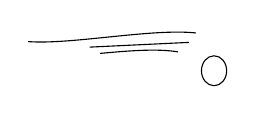
\begin{tikzpicture}[x=1cm,y=1cm]
\draw (0,.26)..controls (.55,.22) and (1.57,.43)..(2.13,.37);
\draw (.78,.19)--(2.04,.25);
\draw (.91,.11)..controls (1.34,.15) and (1.65,.17)..(1.90,.13);
\draw (2.36,-.11) ellipse (.16 and .19);
\end{tikzpicture}}

Soit $\Lambda$ une algèbre $k$-augmentée dont l'idéal
d'augmentation est \deleted{nilpotent}\inserted{de puiss. n.ième nulle}, $k$ étant une
algèbre contenant $\mathbb Q$\inserted{[donc $\Lambda$ contient $\mathbb Q$]}, Soit $M$ un $\Lambda$-module.
Alors les $u\in L_\Lambda(M)$ tels que $uM\subset I(\Lambda)M$
\inserted{i.e. $u$ induit $0$ dans $M\otimes_\Lambda k$}
sont nilpotents \deleted{\unsure{et les sont}}\inserted{(de puiss. n:ième nulle)} les
$v\in L_\Lambda^{\unsure{*|\times}}(M)$ tels que $v$ induise l'identité
dans $M\otimes_\Lambda k$ sont unipotents ; si \unsure{l'ens|l'ens.}
des uns et des autres est $\unsure{\pi^\ell_a|\pi_a}$ resp$^{\mathrm t}$ $\gamma$,
% archive sheet number: 13

\scanpage{15}
on obtient des bijections inverses l'une de l'autre
\diagram{\begin{tikzcd}[ampersand replacement=\&]
\pi\arrow[r,shift left,"\exp"] \& \gamma\arrow[l,shift left,"\log"]
\end{tikzcd}}

Bien entendu, $\pi$ est un idéal \inserted{(nilpotent)} de $L_\Lambda(M)$, et
à fortiori une sous-algèbre de Lie. En
transportant à $\pi$ la structure de groupe de
$\gamma$, on trouve une structure de groupe dans
$\pi$, qui se déduit de sa structure
d'algèbre de Lie par la formule de
Hausdorff-Campbell. Si $M$ est une
$\Lambda$-algèbre \inserted{$\deleted{A}B$}, on trouve le
\uline{corollaire} les \uline{automorphismes} de la
$\Lambda$-algèbre $\underline{\deleted{A}B}$ (où $\Lambda$ est une algèbre
$k$-augmentée à \deleted{\unsure{noyau}} idéal d'augmentation
nilpotent, $k$ étant une $\mathbb Q$-algèbre)
qui induisent l'identité sur $\deleted{\unsure{A}}B\otimes_\Lambda k$
correspondent biunivoquement aux
$\Lambda$-dérivations \inserted{$D$} de $B$ telles que $DB\subset I(\Lambda)B$.
% archive sheet number: 14

\scanpage{16}
Supposons en particulier
\[
B=A\otimes_k\Lambda
\]
où $\Lambda$ est une $k$-algèbre infinitésimale.
Alors \deleted{\unsure{on a} $\Omega^1_{\Lambda}$}
\[
\begin{aligned}
\unsure{\mathfrak g|\mathfrak T|\mathscr T|\mathcal T}_{B/\Lambda}\deleted{(B/\unsure{\Lambda|A})}
&=\mathrm{Hom}_B(\Omega^1_{B/\Lambda},B)\simeq\mathrm{Hom}_B(\Omega^1_{A/k}\otimes_k\Lambda,A\otimes_k\Lambda)\\
&\simeq\mathrm{Hom}_A(\Omega^1_{A/k},A\otimes_k\Lambda)\simeq k\text{-dérivations}\\
&\hspace{14em}\text{de }A\text{ dans }A\otimes_k\Lambda
\end{aligned}
\]
et les $\Lambda$-dérivations de $B$ dans $B$ qui
induisent $0$ sur $B\otimes_\Lambda k\simeq\Lambda$ s'identifient
aux $k$-dérivations $A\unsure{\text{—}|\longrightarrow} A\otimes_k I(\Lambda)$.

Donc

\uline{Proposition} Supposons $k$ \deleted{\unsure{de car.}} $\inserted{\supset}\mathbb Q$, $A$ une
\reversemarginpar\margin{\hfill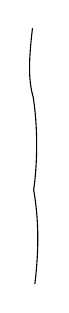
\begin{tikzpicture}[x=3mm,y=5mm]
\draw (0,0) .. controls (-.18,-.9) and (-.16,-1.35) .. (.03,-1.75) .. controls (.30,-2.80) and (.13,-3.80) .. (.05,-4.10) .. controls (.20,-4.65) and (.33,-5.35) .. (.10,-6.5);
\end{tikzpicture}}\normalmarginpar
$k$-alg. comm., $\Lambda$ une $k$-alg. \unsure{diff.|dpf.}
Alors le \inserted{groupe des} $\Lambda$-aut.m. infinitésimaux de
$A\otimes_k\Lambda$ \deleted{\unsure{sont en co}} est isomorphe
à l'ens des $k$-dérivations de
$A$ dans $A\otimes_k I(\Lambda)$, avec la structure
de groupe donnée par Hausdorff-Campbell.
% archive sheet number: 15

